\documentclass[11pt,compress,t,notes=noshow, xcolor=table]{beamer}
\usepackage[]{graphicx}\usepackage[]{color}
% maxwidth is the original width if it is less than linewidth
% otherwise use linewidth (to make sure the graphics do not exceed the margin)
\makeatletter
\def\maxwidth{ %
  \ifdim\Gin@nat@width>\linewidth
    \linewidth
  \else
    \Gin@nat@width
  \fi
}
\makeatother

\definecolor{fgcolor}{rgb}{0.345, 0.345, 0.345}
\newcommand{\hlnum}[1]{\textcolor[rgb]{0.686,0.059,0.569}{#1}}%
\newcommand{\hlstr}[1]{\textcolor[rgb]{0.192,0.494,0.8}{#1}}%
\newcommand{\hlcom}[1]{\textcolor[rgb]{0.678,0.584,0.686}{\textit{#1}}}%
\newcommand{\hlopt}[1]{\textcolor[rgb]{0,0,0}{#1}}%
\newcommand{\hlstd}[1]{\textcolor[rgb]{0.345,0.345,0.345}{#1}}%
\newcommand{\hlkwa}[1]{\textcolor[rgb]{0.161,0.373,0.58}{\textbf{#1}}}%
\newcommand{\hlkwb}[1]{\textcolor[rgb]{0.69,0.353,0.396}{#1}}%
\newcommand{\hlkwc}[1]{\textcolor[rgb]{0.333,0.667,0.333}{#1}}%
\newcommand{\hlkwd}[1]{\textcolor[rgb]{0.737,0.353,0.396}{\textbf{#1}}}%
\let\hlipl\hlkwb

\usepackage{framed}
\makeatletter
\newenvironment{kframe}{%
 \def\at@end@of@kframe{}%
 \ifinner\ifhmode%
  \def\at@end@of@kframe{\end{minipage}}%
  \begin{minipage}{\columnwidth}%
 \fi\fi%
 \def\FrameCommand##1{\hskip\@totalleftmargin \hskip-\fboxsep
 \colorbox{shadecolor}{##1}\hskip-\fboxsep
     % There is no \\@totalrightmargin, so:
     \hskip-\linewidth \hskip-\@totalleftmargin \hskip\columnwidth}%
 \MakeFramed {\advance\hsize-\width
   \@totalleftmargin\z@ \linewidth\hsize
   \@setminipage}}%
 {\par\unskip\endMakeFramed%
 \at@end@of@kframe}
\makeatother

\definecolor{shadecolor}{rgb}{.97, .97, .97}
\definecolor{messagecolor}{rgb}{0, 0, 0}
\definecolor{warningcolor}{rgb}{1, 0, 1}
\definecolor{errorcolor}{rgb}{1, 0, 0}
\newenvironment{knitrout}{}{} % an empty environment to be redefined in TeX

\usepackage{alltt}
\newcommand{\SweaveOpts}[1]{}  % do not interfere with LaTeX
\newcommand{\SweaveInput}[1]{} % because they are not real TeX commands
\newcommand{\Sexpr}[1]{}       % will only be parsed by R



\usepackage[english]{babel}
\usepackage[utf8]{inputenc}

\usepackage{dsfont}
\usepackage{verbatim}
\usepackage{amsmath}
\usepackage{amsfonts}
\usepackage{bm}
\usepackage{csquotes}
\usepackage{multirow}
\usepackage{longtable}
\usepackage{booktabs}
\usepackage{enumerate}
\usepackage[absolute,overlay]{textpos}
\usepackage{psfrag}
\usepackage{algorithm}
\usepackage{algpseudocode}
\usepackage{eqnarray}
\usepackage{arydshln}
\usepackage{tabularx}
\usepackage{placeins}
\usepackage{tikz}
\usepackage{setspace}
\usepackage{colortbl}
\usepackage{mathtools}
\usepackage{wrapfig}
\usepackage{bm}
\usetikzlibrary{shapes,arrows,automata,positioning,calc,chains,trees, shadows}
\tikzset{
  %Define standard arrow tip
  >=stealth',
  %Define style for boxes
  punkt/.style={
    rectangle,
    rounded corners,
    draw=black, very thick,
    text width=6.5em,
    minimum height=2em,
    text centered},
  % Define arrow style
  pil/.style={
    ->,
    thick,
    shorten <=2pt,
    shorten >=2pt,}
}
\usepackage{subfig}


% Defines macros and environments

% basic latex stuff
\newcommand{\pkg}[1]{{\fontseries{b}\selectfont #1}} %fontstyle for R packages
\newcommand{\lz}{\vspace{0.5cm}} %vertical space
\newcommand{\dlz}{\vspace{1cm}} %double vertical space
\newcommand{\mat}[1]{ %short pmatrix command
  \begin{pmatrix}
    #1
  \end{pmatrix}
}
\newcommand{\oneliner}[1] % Oneliner for important statements
{\begin{block}{}\begin{center}\begin{Large}#1\end{Large}\end{center}\end{block}}


% 
% basic latex stuff
\newcommand{\pkg}[1]{{\fontseries{b}\selectfont #1}} %fontstyle for R packages
\newcommand{\lz}{\vspace{0.5cm}} %vertical space
\newcommand{\dlz}{\vspace{1cm}} %double vertical space
\newcommand{\mat}[1]{ %short pmatrix command
  \begin{pmatrix}
    #1
  \end{pmatrix}
}
\newcommand{\oneliner}[1] % Oneliner for important statements
{\begin{block}{}\begin{center}\begin{Large}#1\end{Large}\end{center}\end{block}}



%\usetheme{lmu-lecture}
\usepackage{../../style/lmu-lecture}

\let\code=\texttt
\let\proglang=\textsf

\setkeys{Gin}{width=0.9\textwidth}

\title{Introduction to Machine Learning}
% \author{Bernd Bischl, Christoph Molnar, Daniel Schalk, Fabian Scheipl}
\institute{\href{https://compstat-lmu.github.io/lecture_i2ml/}{compstat-lmu.github.io/lecture\_i2ml}}
\date{}

\setbeamertemplate{frametitle}{\expandafter\uppercase\expandafter\insertframetitle}



\begin{document}


% This file loads R packages, configures knitr options and sets preamble.Rnw as parent file
% IF YOU MODIFY THIS, PLZ ALSO MODIFY setup.Rmd ACCORDINGLY...







% Defines macros and environments
% math spaces
\newcommand{\N}{\mathds{N}}                                                 % N, naturals
\newcommand{\Z}{\mathds{Z}}                                                 % Z, integers
\newcommand{\Q}{\mathds{Q}}                                                 % Q, rationals
\newcommand{\R}{\mathds{R}}                                                 % R, reals
\newcommand{\C}{\mathds{C}}                                                 % C, complex
\newcommand{\HS}{\mathcal{H}}                                               % H, hilbertspace
\newcommand{\continuous}{\mathcal{C}}                                       % C, space of continuous functions
\newcommand{\M}{\mathcal{M}} 												% machine numbers
\newcommand{\epsm}{\epsilon_m} 												% maximum error


% basic math stuff
\newcommand{\xt}{\tilde x}													% x tilde
\def\argmax{\mathop{\sf arg\,max}}                                          % argmax
\def\argmin{\mathop{\sf arg\,min}}                                          % argmin
\newcommand{\sign}{\operatorname{sign}}                                     % sign, signum
\newcommand{\I}{\mathbb{I}}                                                 % I, indicator
\newcommand{\order}{\mathcal{O}}                                            % O, order
\newcommand{\fp}[2]{\frac{\partial #1}{\partial #2}}                        % partial derivative
\newcommand{\pd}[2]{\frac{\partial{#1}}{\partial #2}}						% partial derivative

% sums and products
\newcommand{\sumin}{\sum_{i=1}^n}											% summation from i=1 to n
\newcommand{\sumkg}{\sum_{k=1}^g}											% summation from k=1 to g
\newcommand{\prodin}{\prod_{i=1}^n}											% product from i=1 to n
\newcommand{\prodkg}{\prod_{k=1}^g}											% product from k=1 to g

% linear algebra
\newcommand{\one}{\boldsymbol{1}}                                           % 1, unitvector
\newcommand{\id}{\mathrm{I}}                                                % I, identity
\newcommand{\diag}{\operatorname{diag}}                                     % diag, diagonal
\newcommand{\trace}{\operatorname{tr}}                                      % tr, trace
\newcommand{\spn}{\operatorname{span}}                                      % span
\newcommand{\scp}[2]{\left\langle #1, #2 \right\rangle}                     % <.,.>, scalarproduct
\newcommand{\mat}[1]{ 														% short pmatrix command
	\begin{pmatrix}
		#1
	\end{pmatrix}
}
\newcommand{\Amat}{\bm{A}}													% matrix A
\newcommand{\xv}{\bm{x}}													% vector x (bold)
\newcommand{\yv}{\bm{y}}														% vector y (bold)
\newcommand{\Deltab}{\bm{\Delta}}											% error term for vectors
															

% basic probability + stats
\renewcommand{\P}{\mathds{P}}                                               % P, probability
\newcommand{\E}{\mathds{E}}                                                 % E, expectation
\newcommand{\var}{\mathsf{Var}}                                             % Var, variance
\newcommand{\cov}{\mathsf{Cov}}                                             % Cov, covariance
\newcommand{\corr}{\mathsf{Corr}}                                           % Corr, correlation
\newcommand{\normal}{\mathcal{N}}                                           % N of the normal distribution
\newcommand{\iid}{\overset{i.i.d}{\sim}}                                    % dist with i.i.d superscript
\newcommand{\distas}[1]{\overset{#1}{\sim}}                                 % ... is distributed as ... 
% machine learning

%%%%%% ml - data
\newcommand{\Xspace}{\mathcal{X}}                                           % X, input space
\newcommand{\Yspace}{\mathcal{Y}}                                           % Y, output space
\newcommand{\nset}{\{1, \ldots, n\}}                                        % set from 1 to n
\newcommand{\pset}{\{1, \ldots, p\}}                                        % set from 1 to p
\newcommand{\gset}{\{1, \ldots, g\}}                                        % set from 1 to g
\newcommand{\Pxy}{\P_{xy}}                                                  % P_xy
\newcommand{\xy}{(x, y)}                                                    % observation (x, y)
\newcommand{\xvec}{(x_1, \ldots, x_p)^T}                                    % (x1, ..., xp) 
\newcommand{\D}{\mathcal{D}}                                                % D, data 
\newcommand{\Dset}{\{ (x^{(1)}, y^{(1)}), \ldots, (x^{(n)},  y^{(n)})\}}    % {(x1,y1)), ..., (xn,yn)}, data
\newcommand{\xdat}{\{ x^{(1)}, \ldots, x^{(n)}\}}   						 % {x1, ..., xn}, input data
\newcommand{\ydat}{\mathbf{y}}                                              % y (bold), vector of outcomes
\newcommand{\yvec}{(y^{(1)}, \hdots, y^{(n)})^T}                            % (y1, ..., yn), vector of outcomes
\renewcommand{\xi}[1][i]{x^{(#1)}}                                          % x^i, i-th observed value of x
\newcommand{\yi}[1][i]{y^{(#1)}}                                            % y^i, i-th observed value of y 
\newcommand{\xyi}{(\xi, \yi)}                                               % (x^i, y^i), i-th observation
\newcommand{\xivec}{(x^{(i)}_1, \ldots, x^{(i)}_p)^T}                       % (x1^i, ..., xp^i), i-th observation vector
\newcommand{\xj}{x_j}                                                       % x_j, j-th feature
\newcommand{\xjb}{\mathbf{x}_j}                                             % x_j (bold), j-th feature vecor
\newcommand{\xjvec}{(x^{(1)}_j, \ldots, x^{(n)}_j)^T}                       % (x^1_j, ..., x^n_j), j-th feature vector
\newcommand{\Dtrain}{\mathcal{D}_{\text{train}}}                            % D_train, training set
\newcommand{\Dtest}{\mathcal{D}_{\text{test}}}                              % D_test, test set

%%%%%% ml - models general

% continuous prediction function f
\newcommand{\fx}{f(x)}                                                      % f(x), continuous prediction function
\newcommand{\Hspace}{H}														% hypothesis space where f is from
\newcommand{\fh}{\hat{f}}                                                   % f hat, estimated prediction function
\newcommand{\fxh}{\fh(x)}                                                   % fhat(x)
\newcommand{\fxt}{f(x | \theta)}                                            % f(x | theta)
\newcommand{\fxi}{f(\xi)}                                                   % f(x^(i))
\newcommand{\fxih}{\hat{f}(\xi)}                                            % f(x^(i))
\newcommand{\fxit}{f(x^{(i)} | \theta)}                                     % f(x^(i) | theta)
\newcommand{\fhD}{\fh_{\D}}                                                 % fhat_D, estimate of f based on D
\newcommand{\fhDtrain}{\fh_{\Dtrain}}                                       % fhat_Dtrain, estimate of f based on D

% discrete prediction function h
\newcommand{\hx}{h(x)}                                                      % h(x), discrete prediction function
\newcommand{\hh}{\hat{h}}                                                   % h hat
\newcommand{\hxh}{\hat{h}(x)}                                               % hhat(x)
\newcommand{\hxt}{h(x | \theta)}                                            % h(x | theta)
\newcommand{\hxi}{h(\xi)}                                                   % h(x^(i))
\newcommand{\hxit}{h(x^{(i)} | \theta)}                                     % h(x^(i) | theta)

% yhat
\newcommand{\yh}{\hat{y}}                                                   % y hat for prediction of target
\newcommand{\yih}{\hat{y}}                                                  % y hat for prediction of target

% theta
\newcommand{\thetah}{\hat{\theta}}                                          % theta hat

% densities + probabilities
% pdf of x 
\newcommand{\pdf}{p}                                                        % p
\newcommand{\pdfx}{p(x)}                                                    % p(x)
\newcommand{\pixt}{\pi(x | \theta)}                                         % pi(x|theta), pdf of x given theta

% pdf of (x, y)
\newcommand{\pdfxy}{p(x,y)}                                                 % p(x, y)
\newcommand{\pdfxyt}{p(x, y | \theta)}                                      % p(x, y | theta)
\newcommand{\pdfxyit}{p(\xi, \yi | \theta)}                                 % p(x^(i), y^(i) | theta)

% pdf of x given y
\newcommand{\pdfxyk}{p(x | y=k)}                                            % p(x | y = k)
\newcommand{\lpdfxyk}{\log \pdfxyk}                                         % log p(x | y = k)
\newcommand{\pdfxiyk}{p(\xi | y=k)}                                         % p(x^i | y = k)

% prior probabilities
\newcommand{\pik}{\pi_k}                                                    % pi_k, prior
\newcommand{\lpik}{\log \pik}                                               % log pi_k, log of the prior

% posterior probabilities
\newcommand{\post}{\P(y = 1 | x)}                                           % P(y = 1 | x), post. prob for y=1
\newcommand{\pix}{\pi(x)}                                                   % pi(x), P(y = 1 | x)
\newcommand{\postk}{\P(y = k | x)}                                          % P(y = k | y), post. prob for y=k
\newcommand{\pikx}{\pi_k(x)}                                                % pi_k(x), P(y = k | x)
\newcommand{\pikxt}{\pi_k(x | \theta)}                                      % pi_k(x | theta), P(y = k | x, theta)
\newcommand{\pijx}{\pi_j(x)}                                                % pi_j(x), P(y = j | x)
\newcommand{\pdfygxt}{p(y |x, \theta)}                                      % p(y | x, theta)
\newcommand{\pdfyigxit}{p(\yi |\xi, \theta)}                                % p(y^i |x^i, theta)
\newcommand{\lpdfygxt}{\log \pdfygxt }                                      % log p(y | x, theta)
\newcommand{\lpdfyigxit}{\log \pdfyigxit}                                   % log p(y^i |x^i, theta)
\newcommand{\pixh}{\hat \pi(x)}                                             % pi(x) hat, P(y = 1 | x) hat
\newcommand{\pikxh}{\hat \pi_k(x)}                                          % pi_k(x) hat, P(y = k | x) hat

% residual and margin
\newcommand{\eps}{\epsilon}                                                 % residual, stochastic
\newcommand{\epsi}{\epsilon^{(i)}}                                          % epsilon^i, residual, stochastic
\newcommand{\epsh}{\hat{\epsilon}}                                          % residual, estimated
\newcommand{\yf}{y \fx}                                                     % y f(x), margin
\newcommand{\yfi}{\yi \fxi}                                                 % y^i f(x^i), margin
\newcommand{\Sigmah}{\hat \Sigma}											% estimated covariance matrix
\newcommand{\Sigmahj}{\hat \Sigma_j}										% estimated covariance matrix for the j-th class

% ml - loss, risk, likelihood
\newcommand{\Lxy}{L(y, f(x))}                                               % L(y, f(x)), loss function
\newcommand{\Lxyi}{L(\yi, \fxi)}                                            % L(y^i, f(x^i))
\newcommand{\Lxyt}{L(y, \fxt)}                                              % L(y, f(x | theta))
\newcommand{\Lxyit}{L(\yi, \fxit)}                                          % L(y^i, f(x^i | theta)
\newcommand{\risk}{\mathcal{R}}                                             % R, risk
\newcommand{\riskf}{\risk(f)}                                               % R(f), risk
\newcommand{\riske}{\mathcal{R}_{\text{emp}}}                               % R_emp, empirical risk
\newcommand{\riskef}{\riske(f)}                                             % R_emp(f)
\newcommand{\risket}{\mathcal{R}_{\text{emp}}(\theta)}                      % R_emp(theta)
\newcommand{\riskr}{\mathcal{R}_{\text{reg}}}                               % R_reg, regularized risk
\newcommand{\riskrt}{\mathcal{R}_{\text{reg}}(\theta)}                      % R_reg(theta)
\newcommand{\riskrf}{\riskr(f)}                                             % R_reg(f)
\newcommand{\LL}{\mathcal{L}}                                               % L, likelihood
\newcommand{\LLt}{\mathcal{L}(\theta)}                                      % L(theta), likelihood
\renewcommand{\ll}{\ell}                                                    % l, log-likelihood
\newcommand{\llt}{\ell(\theta)}                                             % l(theta), log-likelihood
\newcommand{\LS}{\mathfrak{L}}                                              % ????????????
\newcommand{\TS}{\mathfrak{T}}                                              % ??????????????
\newcommand{\errtrain}{\text{err}_{\text{train}}}                           % training error
\newcommand{\errtest}{\text{err}_{\text{test}}}                             % training error
\newcommand{\errexp}{\overline{\text{err}_{\text{test}}}}                   % training error

% resampling
\newcommand{\GE}[1]{GE(\fh_{#1})}                                           % Generalization error GE
\newcommand{\GEh}[1]{\widehat{GE}_{#1}}                                     % Estimated train error
\newcommand{\GED}{\GE{\D}}                                                  % Generalization error GE
\newcommand{\EGEn}{EGE_n}                                                   % Generalization error GE
\newcommand{\EDn}{\E_{|D| = n}}                                             % Generalization error GE


% ml - irace
\newcommand{\costs}{\mathcal{C}} % costs
\newcommand{\Celite}{\theta^*} % elite configurations
\newcommand{\instances}{\mathcal{I}} % sequence of instances
\newcommand{\budget}{\mathcal{B}} % computational budget
%! includes: evaluation-measures-classification

\lecturechapter{Evaluation: Measures for Binary Classification: ROC Measures}
\lecture{Introduction to Machine Learning}

\begin{vbframe}{Imbalanced Binary Labels}

\begin{center}
% FIGURE SOURCE: https://docs.google.com/drawings/d/1WERS9WXwS4zla86fk6ESQkskNN1WZMI1YCPprnp0Ew0/edit?usp=sharing

\includegraphics[width=.9\textwidth]{figure_man/imbalanced.pdf}\\
Classify all as \enquote{no disease} (green) $\rightarrow$ high accuracy.

\lz

\textbf{Accuracy Paradox}
\end{center}

\end{vbframe}


\begin{vbframe}{Imbalanced Costs}

\begin{center}
% FIGURE SOURCE: https://docs.google.com/drawings/d/1GlmMqzpeNHU_rtPFIrJMlY9Iz6XexvHEwTl3dNYKyQU/edit?usp=sharing
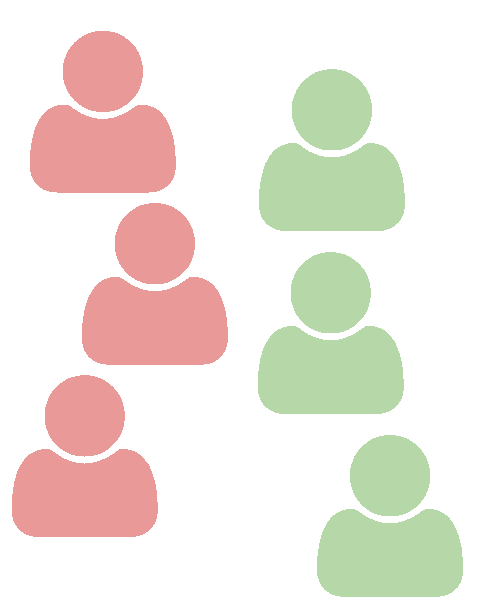
\includegraphics[width=.3\textwidth]{figure_man/imbalanced-costs.pdf}\\
Classify incorrectly as \enquote{no disease} $\rightarrow$ very high cost

\end{center}

\end{vbframe}

% \begin{vbframe}{Imbalanced Binary Labels}
% \begin{itemize}
%   \item Consider a binary classifier for diagnosing a serious medical condition
%   \item Here, label distribution is often \textbf{imbalanced}, i.e, not many people have the disease
%   \item Evaluating with error rate for imbalanced labels is often inappropriate
%   \item Assume that only 0.5\,\% of 1000 patients have the disease
%   \item Always returning "no disease" has an error rate of 0.5\,\%, which sounds good
%   \item However, this sends all sick patients home, which is the worst possible system, even classifying everyone as "sick" might be better, depending on what happens next
%   \item This problem is sometimes known as the \textbf{accuracy paradox}
% \end{itemize}
% \end{vbframe}
% 
% \begin{vbframe}{Binary Classifiers and Costs}
% \begin{itemize}
%   \item Another point of view is imbalanced costs
%   \item In our example, classifying a sick patient as healthy, should incur a much higher loss then classifying a healthy patient as sick
%   \item The costs depend a lot on what happens next: We can likely assume that our system is some type of screening filter,
%     often the next step after labeling someone as "sick" might be a more invasive, expensive, but more reliable test for the disease
%   \item Erroneously subjecting someone to that second step is not good (psychologically, economically, or because the second test might introduce
%     medical risks), but sending someone home to get worse or die seems much worse
%   \item Such a situation not only arises under label imbalance, but also when labels are maybe balanced but costs differ
%   \item We could see this as imbalanced costs of misclassification, rather than imbalanced labels; both situations are tightly connected
% \end{itemize}
% \end{vbframe}
% 
% \begin{vbframe}{Binary Classifiers and Costs}
% \begin{itemize}
%   \item Problem is: If we could specify costs precisely, we could evaluate against them, we might even optimize our model for them
%   \item This important subfield of ML is called \textbf{cost-sensitive learning}, which we will not cover in this lecture unit
%   \item Unfortunately, users often have a notoriously hard time to come up with precise cost numbers in imbalanced scenarios
%   \item Evaluating "from different perspectives", with multiple metrics, often helps, especially to get a first impression
%     of the quality of the system
% \end{itemize}
% \end{vbframe}
% 

% 
% 
% \begin{vbframe}{Confusion Matrix and ROC Metrics}
% \begin{itemize}
%   \item From now on, we call one class "positive", one "negative" and their respective sizes
%     $n_+$ and $n_-$
%   \item The positive class is the more important, often smaller one
%   \item We represent all predictions in a confusion matrix and count correct and incorrect class assignments
%   \item False Positive means: We assigned "positive", but were wrong
% \end{itemize}
% % FIGURE SOURCE: No source
% 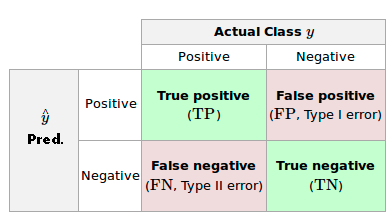
\includegraphics[width=0.7\textwidth]{figure_man/roc-confmatrix1.png}
% \end{vbframe}


\begin{vbframe}{Confusion Matrix}

\begin{center}
\small
\renewcommand{\arraystretch}{1.5}
\begin{tabular}{cc||cc}
    & & \multicolumn{2}{c}{\bfseries True Class $y$}  \\
    & & $+$ & $-$  \\ 
    \hline \hline
    \bfseries Pred.     & $+$ & TP & FP\\
              $\yh$ & $-$ & FN & TN\\ 
\end{tabular}
\renewcommand{\arraystretch}{1}
\end{center}

\begin{itemize}
  \item $+$: \enquote{positive} class
  \item $-$: \enquote{negative} class
  \item $\np$: number of observations in $+$
  \item $\nn$: number of observations in $-$
\end{itemize}
\end{vbframe}


\begin{vbframe}{Labels: ROC Metrics}
From the confusion matrix (binary case), we can calculate "ROC" metrics.

% % FIGURE SOURCE: No source
% 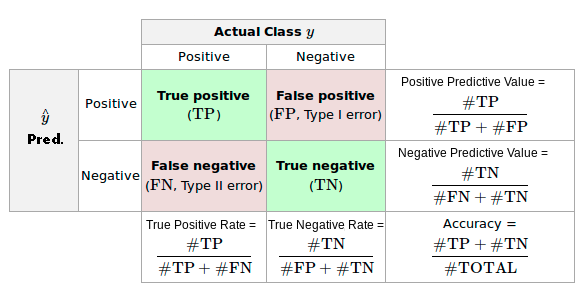
\includegraphics[width=0.7\textwidth]{figure_man/roc-confmatrix2.png}

% \begin{center}
% \small
% \begin{tabular}{cc|>{\centering\arraybackslash}p{7em}>{\centering\arraybackslash}p{8em}|>{\centering\arraybackslash}p{8em}}
%     & & \multicolumn{2}{c}{\bfseries True Class $y$} & \\
%     & & $+$ & $-$ & \\
%     \hline
%     \bfseries Pred.     & $+$ & True Positive (TP)  & False Positive (FP) & Positive Predictive Value (PPV) = $\frac{\text{TP}}{\text{TP} + \text{FP}}$\\
%               $\hat{y}$ & $-$ & False Negative (FN) & True Negative (TN) & Negative Predictive Value (NPV) = $\frac{\text{TN}}{\text{FN} + \text{TN}}$\\
%     \hline
%     & & TPR = $\frac{\text{TP}}{\text{TP} + \text{FN}}$ & TNR = $\frac{\text{TN}}{\text{FP} + \text{TN}}$ & Accuracy = $\frac{\text{TP}+ \text{TN}}{\text{TOTAL}}$
% \end{tabular}
% \end{center}

\begin{center}
\small
\renewcommand{\arraystretch}{1.5}
\begin{tabular}{cc||cc|c}
    & & \multicolumn{2}{c|}{\bfseries True Class $y$} & \\
    & & $+$ & $-$ & \\ 
    \hline \hline
    \bfseries Pred.     & $+$ & TP & FP & PPV = $\frac{\text{TP}}{\text{TP} + \text{FP}}$\\
              $\yh$ & $-$ & FN & TN & NPV = $\frac{\text{TN}}{\text{FN} + \text{TN}}$\\
    \hline
    & & TPR = $\frac{\text{TP}}{\text{TP} + \text{FN}}$ & TNR = $\frac{\text{TN}}{\text{FP} + \text{TN}}$ & Accuracy = $\frac{\text{TP}+ \text{TN}}{\text{TOTAL}}$
\end{tabular}
\renewcommand{\arraystretch}{1}
\end{center}

\begin{itemize}
  \item True Positive Rate: How many of the true 1s did we predict as 1?
  \item True Negative Rate: How many of the true 0s did we predict as 0?
  \item Positive Predictive Value: If we predict 1 how likely is it a true 1?
  \item Negative Predictive Value: If we predict 0 how likely is it a true 0?
\end{itemize}
\end{vbframe}


\begin{frame}{History ROC}
ROC = receiver operating characteristics

\lz

Initially developed by electrical engineers and radar engineers during World War II for detecting enemy objects in battlefields. 

\begin{center}
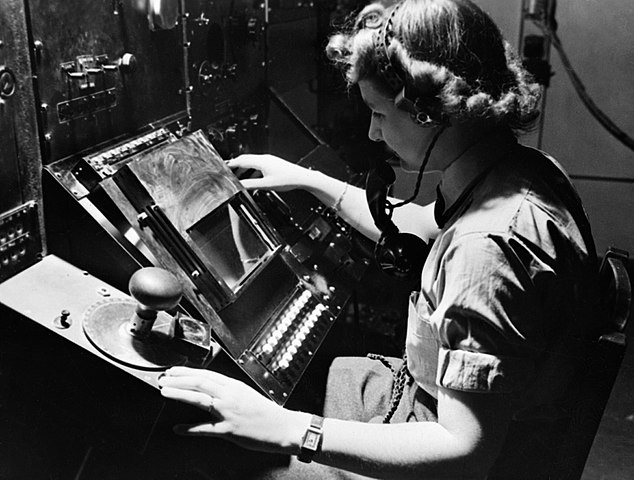
\includegraphics[width=.4\textwidth]{figure_man/receiver_operator.jpg}
{\tiny \url{http://media.iwm.org.uk/iwm/mediaLib//39/media-39665/large.jpg}}
\end{center}

Still has the funny name.
\end{frame}


\begin{vbframe}{Labels: ROC}
Example
\begin{center}
  % FIGURE SOURCE: No source
  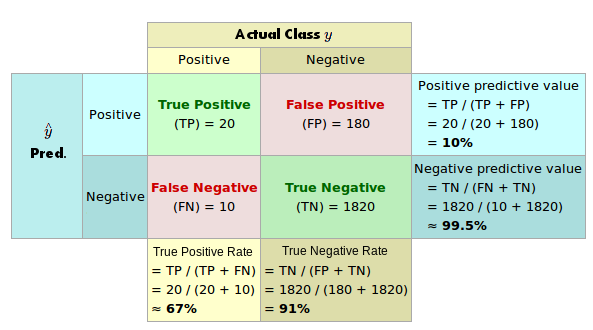
\includegraphics[width=\textwidth]{figure_man/roc-confmatrix-example.png}
\end{center}

\end{vbframe}

\begin{vbframe}{More metrics and alternative terminology}

Unfortunately, for many concepts in ROC, 2-3 different terms exist.

\begin{center}
% FIGURE SOURCE: https://en.wikipedia.org/wiki/F1_score#Diagnostic_testing
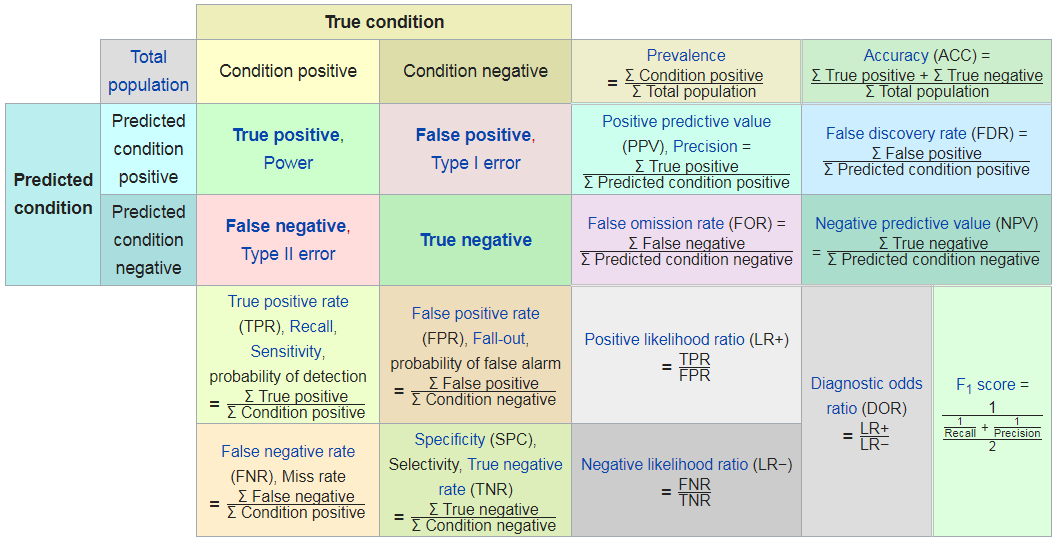
\includegraphics[width=0.95\textwidth]{figure_man/roc-confmatrix-allterms.png}
\end{center}
\href{https://en.wikipedia.org/wiki/F1_score#Diagnostic_testing}{\beamergotobutton{Clickable version/picture source}} $\phantom{blablabla}$
\href{https://upload.wikimedia.org/wikipedia/commons/0/0e/DiagnosticTesting_Diagram.svg}{\beamergotobutton{Interactive diagram}}
\end{vbframe}


\begin{vbframe}{Labels: $F_1$-Measure}

% \begin{itemize}
%   \item It is difficult to achieve a high \textit{Positive Predictive Value} and high \textit{True Positive Rate} simultaneously.
%   \item A classifier that predicts more "positives" will tend to be more sensitive (higher TPR), but it will also tend to give more false positives (lower TNR, lower PPV).
%   \item A classifier that predicts more "negatives" will tend to be more precise (higher PPV), but it will also produce more false negatives (lower TPR).
% \end{itemize}

\lz
A measure that balances two conflicting goals\\[.5em]
\begin{enumerate}
 \item Maximising Positive Predictive Value
 \item Maximising True Positive Rate\\[.5em]
\end{enumerate}
is the harmonic mean of PPV and TPR:
$$F_1 = 2 \cfrac{PPV \cdot TPR}{PPV + TPR}$$

\lz \lz
Note: still doesn’t account for the number of true negatives.
\end{vbframe}

\begin{vbframe}{Labels: $F_1$-Measure}
Tabulated $F_1$-Score for different TPR (rows) and PPV (cols) combinations. 
\begin{knitrout}\scriptsize
\definecolor{shadecolor}{rgb}{0.969, 0.969, 0.969}\color{fgcolor}\begin{kframe}
\begin{verbatim}
    0.0  0.2  0.4  0.6  0.8  1.0
0.0   0 0.00 0.00 0.00 0.00 0.00
0.2   0 0.20 0.27 0.30 0.32 0.33
0.4   0 0.27 0.40 0.48 0.53 0.57
0.6   0 0.30 0.48 0.60 0.69 0.75
0.8   0 0.32 0.53 0.69 0.80 0.89
1.0   0 0.33 0.57 0.75 0.89 1.00
\end{verbatim}
\end{kframe}
\end{knitrout}
$\rightarrow$ Tends more towards the lower of the 2 combined values.


\begin{itemize}
  \item $TPR = 0$ or $PPV=0$ $\Rightarrow$ $F_1$ of 0
  \item Predicting always "neg": $F_1 = 0$
  \item Predicting always "pos": $F_1 = 2 PPV / (PPV + 1) = 2 \np / (\np + n)$,\\ 
  which will be rather small, if the size of the positive class $\np$ is small.
\end{itemize}


\end{vbframe}

\endlecture

\end{document}
